\section{Jao Gap}\label{sec:JaoGap}
A theoretical explanation for the Jao Gap (Figure \ref{fig:JaoGap}) comes from
\citet{van2012}, who propose that in a star directly above the transition mass,
due to asymmetric production and destruction of He$^{3}$ during the
proton-proton I chain (ppI), periodic luminosity variations can be induced.
This process is known as convective-kissing instability. Such a star will
descend the pre-main sequence with a radiative core; however, as the star
reaches the zero age main sequence (ZAMS) and as the core temperature exceeds
$7\times 10^{6}$ K, enough energy will be produced by the ppI chain that the
core becomes convective. At this point the star exists with both a convective
core and envelope, in addition to a thin, radiative, layer separating the two.
Subsequently, asymmetries in ppI affect the evolution of the star's convective
core.

\begin{figure}
	\centering
	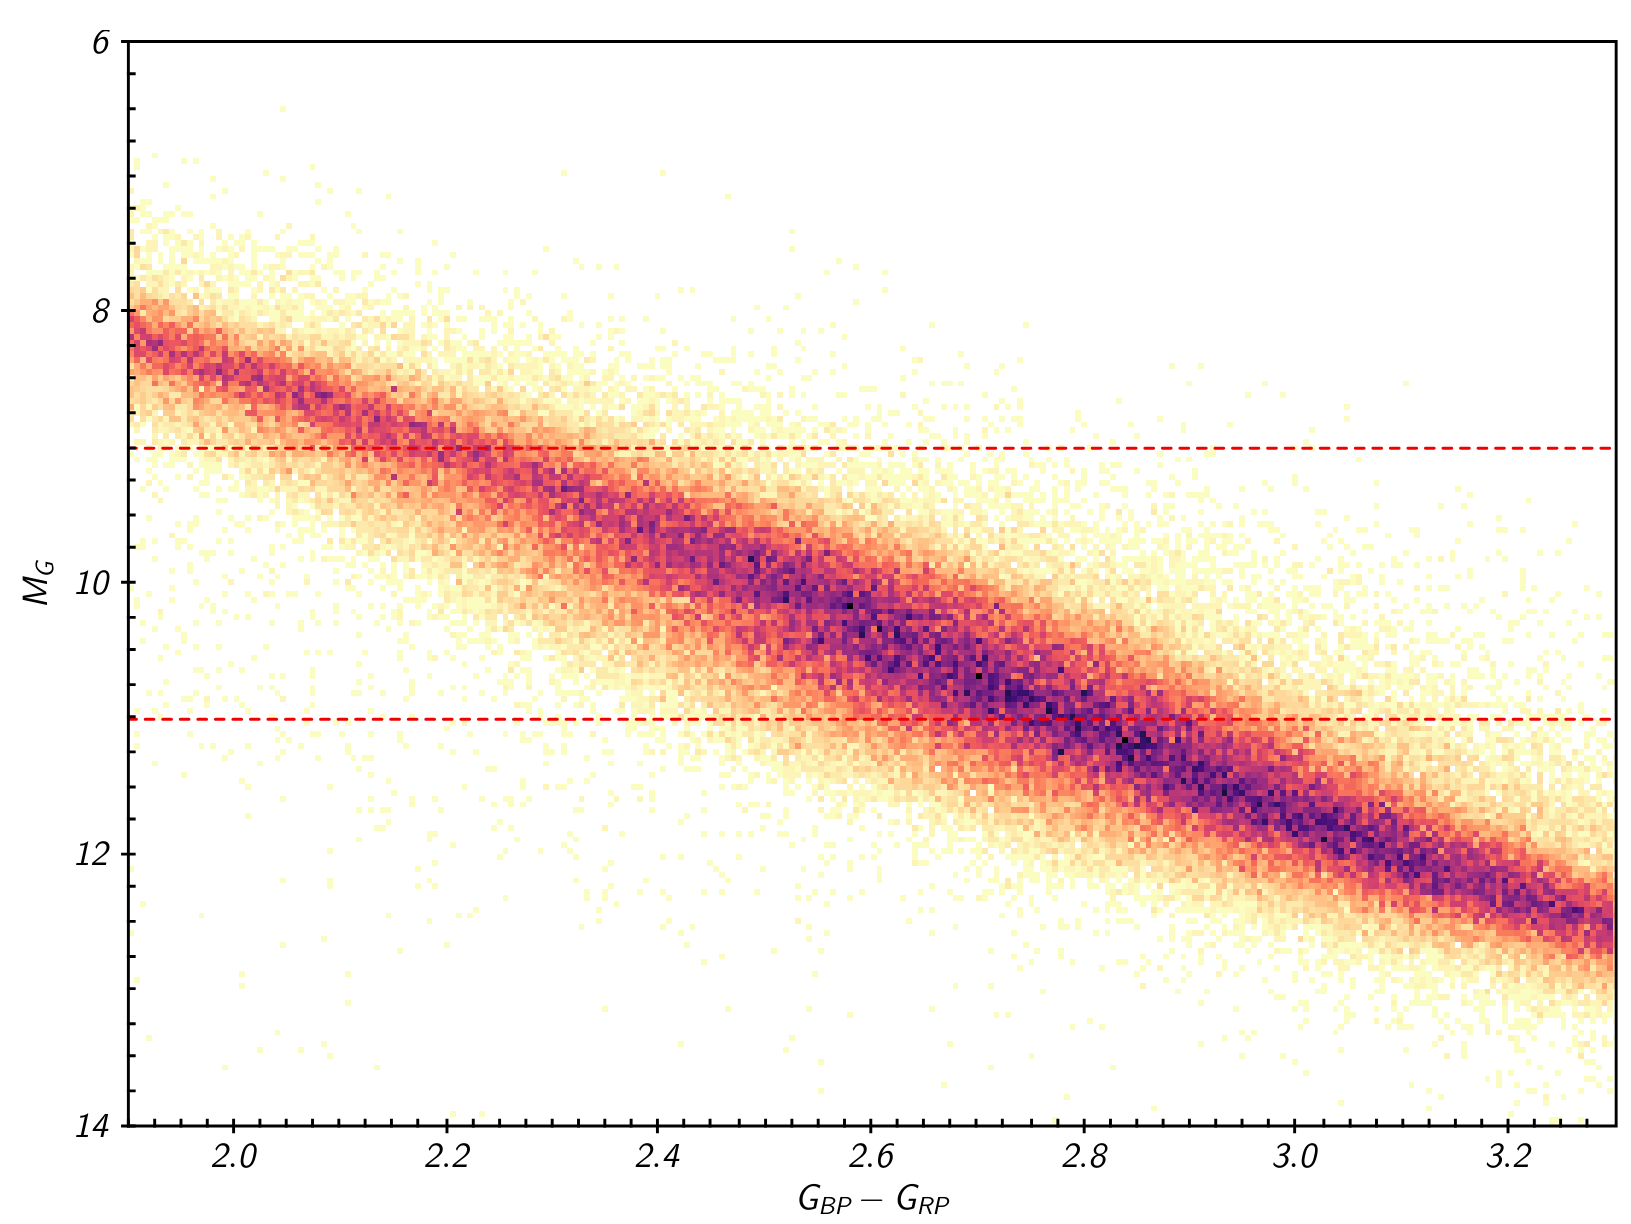
\includegraphics[width=0.45\textwidth]{src/figures/JaoGap.png}
	\caption{Figure 1 from \citet{Jao2018} showing the so called ``Jao Gap'' at
	$M_{G}\approx$ 10 {\color{red} [SHOULD I REMAKE THIS USING DR3 DATA?]}}
	\label{fig:JaoGap}
\end{figure}

The proton-proton I chain constitutes three reactions 
\begin{enumerate} 
	\item $p + p \longrightarrow d + e^{+} + \nu_{e}$
	\item $p + d \longrightarrow \ ^{3}\text{He} + \gamma$
	\item $^{3}\text{He} + ^{3}\text{He} \longrightarrow \ ^{3}\text{He} + 2p$ 
\end{enumerate} 
Because reaction 3 of ppI consumes $^{3}$He at a slower rate than it is
produced by reaction 2, $^{3}$He abundance increases in the core increasing
energy generation. The core convective zone will therefore expand as more of
the star becomes unstable to convection. This expansion will continue until the
core connects with the convective envelope. At this point convective mixing can
transport material throughout the entire radius of the star and the high
concentration of $^{3}$He will rapidly diffuse outward, away from the core,
again decreasing energy generation as reaction 3 slows down. Ultimately, this
leads to the convective region around the core pulling back away from the
convective envelope, leaving in place the radiative transition zone, at which
point $^{3}$He concentrations build up in the core until it once again expands
to meet the envelope.  This process repeats until the He$^{3}$ concentration
throughout the star is enough such that the core can sustain nuclear reaction
rates which keep it in with the envelope, resulting in a fully convective star.


\subsubsection{Modeling the Gap}
Since the identification of the Gaia M-dwarf gap, stellar modeling has been
conducted to better constrain its location, effects, and exact cause.
Both \citet{Mansfield2021} and \citet{Feiden2021} identify that the gap's mass
location is correlated with model metallicity --- the mass-luminosity
discontinuity in lower metallicity models being at a commensurately lower mass.
\citet{Feiden2021} suggests this dependence is due to the steep relation of
the radiative temperature gradient, $\nabla_{rad}$, on temperature and in turn,
on stellar mass.

\begin{align}\label{eqn:radGrad}
	\nabla_{rad} \propto \frac{L\kappa}{T^{4}}
\end{align}

As metallicity decreases so does opacity, which, by Equation \ref{eqn:radGrad},
dramatically lowers the temperature where radiation will dominate energy transport
\citep{Chabrier1997}. Since main sequence stars are virialized the core
temperature is proportional to the core density and total mass (Equation
\ref{eqn:TMRelation}). Therefore, if the core temperature where
convective-kissing instability is expected decreases with metallicity, so too
will the mass of stars which experience such instabilities.

\begin{align}\label{eqn:TMRelation}
	T_{c} \propto \rho_{c}M^{2}
\end{align}

This strong opacity dependence presents a slight problem where modeling is 
concerned. With current computational tools it is infeasible to compute opacities on the
fly; rather, Rossland Mean opacity ($\kappa_{R}$) for individual elements must
be pre-tabulated over a wide range of temperatures and densities. These
opacities can then be somewhat arbitrarily mixed together and interpolated to
form opacity lookup-tables. Multiple groups have performed these calculations
and subsequently made tables available to the wider community, these include
the Opacity Project \citep[OP][]{Seaton1994}, Laurence Livermore National Labs
OPAL opacity tables \citep{Iglesias1996}, and Los Alamos National Labs OPLIB
opacity tables \citep{Colgan2016}.


\begin{figure}
	\centering
	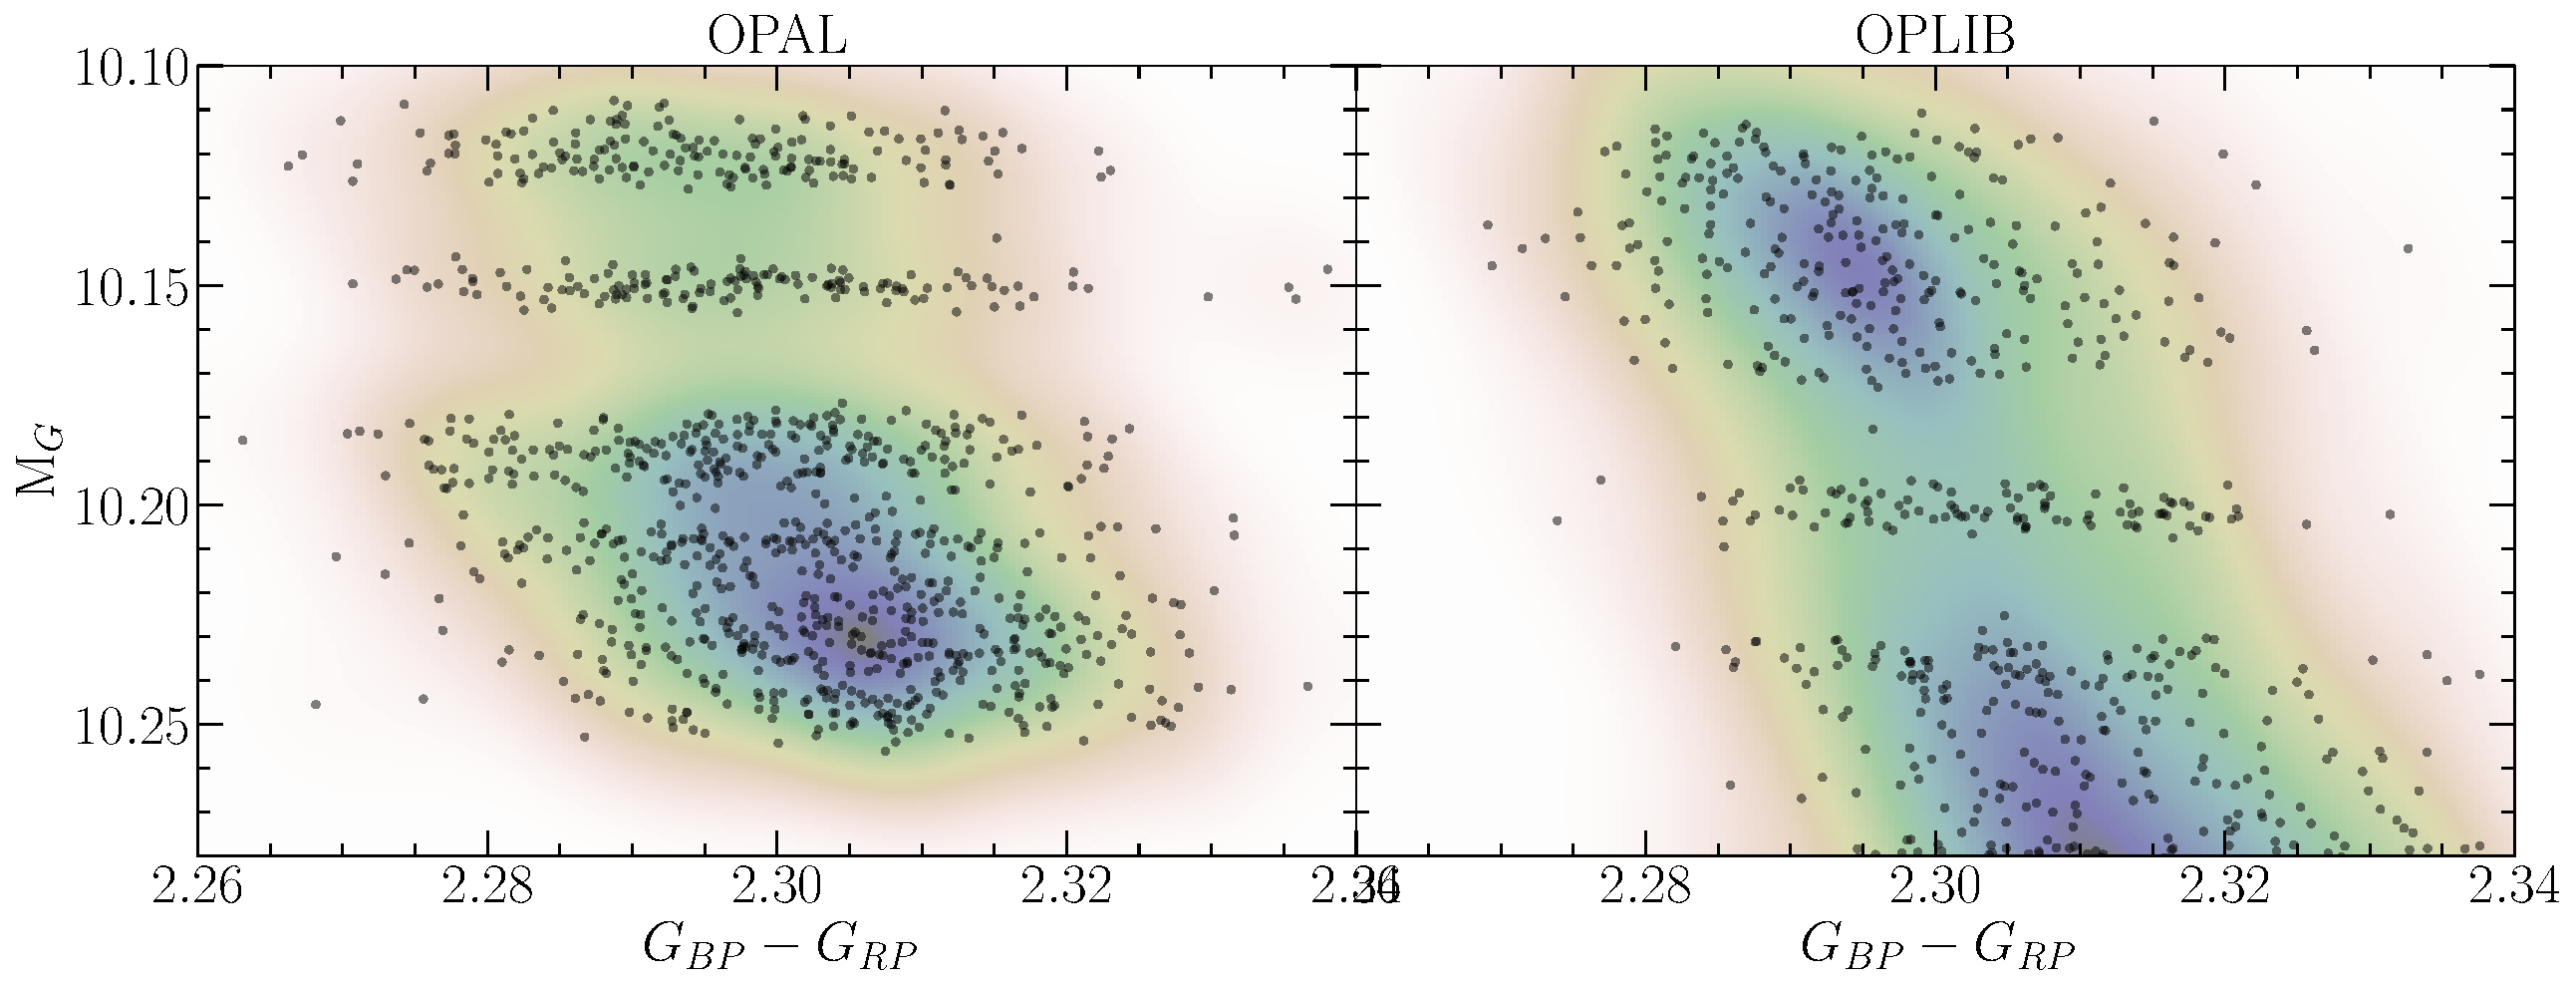
\includegraphics[width=0.45\textwidth]{src/figures/OPALOPLIB_popsynth_comp.pdf}
	\caption{Synthetic CMDs derived from simple population synthesis code.
	(Left) CMD showing the Jao Gap for a GS98 composition stellar population
	generated from models evolved using OPAL opacity tables. (Right) CMD showing
	the Jao Gap for a GS98 stellar population generated from models evolved
	using the OPLIB opacity tables. Note how the OPLIB derived Jao Gap is
	slightly brighter than the OPAL Jao Gap.}
	\label{fig:JaoGapOPALOPLIB}
\end{figure}



\begin{table*}
	\centering
	\begin{tabular}{r | c c c c}
		\hline
		$Z=$ & Z$_{\odot}$ & 0.01 & 0.001 & 0.0001 \\
		\hline
		\hline
		OPAL & 0.3803 - 0.384 & 0.3583 - 0.3631 & 0.34 - 0.3448 & 0.362 - 0.3663 \\
		OPLIB & 0.374 - 0.3767 & 0.3526 - 0.3567 & 0.3358 - 0.3406 & 0.3577 - 0.3621
	\end{tabular}
	\caption{Mass ranges for the discontinuity in OPAL and OPLIB models. Masses
	are given in solar masses.}
	\label{tab:fineMassRange}
\end{table*}
